
% Default to the notebook output style

    


% Inherit from the specified cell style.




    
\documentclass[11pt]{article}

    
    
    \usepackage[T1]{fontenc}
    % Nicer default font (+ math font) than Computer Modern for most use cases
    \usepackage{mathpazo}

    % Basic figure setup, for now with no caption control since it's done
    % automatically by Pandoc (which extracts ![](path) syntax from Markdown).
    \usepackage{graphicx}
    % We will generate all images so they have a width \maxwidth. This means
    % that they will get their normal width if they fit onto the page, but
    % are scaled down if they would overflow the margins.
    \makeatletter
    \def\maxwidth{\ifdim\Gin@nat@width>\linewidth\linewidth
    \else\Gin@nat@width\fi}
    \makeatother
    \let\Oldincludegraphics\includegraphics
    % Set max figure width to be 80% of text width, for now hardcoded.
    \renewcommand{\includegraphics}[1]{\Oldincludegraphics[width=.8\maxwidth]{#1}}
    % Ensure that by default, figures have no caption (until we provide a
    % proper Figure object with a Caption API and a way to capture that
    % in the conversion process - todo).
    \usepackage{caption}
    \DeclareCaptionLabelFormat{nolabel}{}
    \captionsetup{labelformat=nolabel}

    \usepackage{adjustbox} % Used to constrain images to a maximum size 
    \usepackage{xcolor} % Allow colors to be defined
    \usepackage{enumerate} % Needed for markdown enumerations to work
    \usepackage{geometry} % Used to adjust the document margins
    \usepackage{amsmath} % Equations
    \usepackage{amssymb} % Equations
    \usepackage{textcomp} % defines textquotesingle
    % Hack from http://tex.stackexchange.com/a/47451/13684:
    \AtBeginDocument{%
        \def\PYZsq{\textquotesingle}% Upright quotes in Pygmentized code
    }
    \usepackage{upquote} % Upright quotes for verbatim code
    \usepackage{eurosym} % defines \euro
    \usepackage[mathletters]{ucs} % Extended unicode (utf-8) support
    \usepackage[utf8x]{inputenc} % Allow utf-8 characters in the tex document
    \usepackage{fancyvrb} % verbatim replacement that allows latex
    \usepackage{grffile} % extends the file name processing of package graphics 
                         % to support a larger range 
    % The hyperref package gives us a pdf with properly built
    % internal navigation ('pdf bookmarks' for the table of contents,
    % internal cross-reference links, web links for URLs, etc.)
    \usepackage{hyperref}
    \usepackage{longtable} % longtable support required by pandoc >1.10
    \usepackage{booktabs}  % table support for pandoc > 1.12.2
    \usepackage[inline]{enumitem} % IRkernel/repr support (it uses the enumerate* environment)
    \usepackage[normalem]{ulem} % ulem is needed to support strikethroughs (\sout)
                                % normalem makes italics be italics, not underlines
    

    
    
    % Colors for the hyperref package
    \definecolor{urlcolor}{rgb}{0,.145,.698}
    \definecolor{linkcolor}{rgb}{.71,0.21,0.01}
    \definecolor{citecolor}{rgb}{.12,.54,.11}

    % ANSI colors
    \definecolor{ansi-black}{HTML}{3E424D}
    \definecolor{ansi-black-intense}{HTML}{282C36}
    \definecolor{ansi-red}{HTML}{E75C58}
    \definecolor{ansi-red-intense}{HTML}{B22B31}
    \definecolor{ansi-green}{HTML}{00A250}
    \definecolor{ansi-green-intense}{HTML}{007427}
    \definecolor{ansi-yellow}{HTML}{DDB62B}
    \definecolor{ansi-yellow-intense}{HTML}{B27D12}
    \definecolor{ansi-blue}{HTML}{208FFB}
    \definecolor{ansi-blue-intense}{HTML}{0065CA}
    \definecolor{ansi-magenta}{HTML}{D160C4}
    \definecolor{ansi-magenta-intense}{HTML}{A03196}
    \definecolor{ansi-cyan}{HTML}{60C6C8}
    \definecolor{ansi-cyan-intense}{HTML}{258F8F}
    \definecolor{ansi-white}{HTML}{C5C1B4}
    \definecolor{ansi-white-intense}{HTML}{A1A6B2}

    % commands and environments needed by pandoc snippets
    % extracted from the output of `pandoc -s`
    \providecommand{\tightlist}{%
      \setlength{\itemsep}{0pt}\setlength{\parskip}{0pt}}
    \DefineVerbatimEnvironment{Highlighting}{Verbatim}{commandchars=\\\{\}}
    % Add ',fontsize=\small' for more characters per line
    \newenvironment{Shaded}{}{}
    \newcommand{\KeywordTok}[1]{\textcolor[rgb]{0.00,0.44,0.13}{\textbf{{#1}}}}
    \newcommand{\DataTypeTok}[1]{\textcolor[rgb]{0.56,0.13,0.00}{{#1}}}
    \newcommand{\DecValTok}[1]{\textcolor[rgb]{0.25,0.63,0.44}{{#1}}}
    \newcommand{\BaseNTok}[1]{\textcolor[rgb]{0.25,0.63,0.44}{{#1}}}
    \newcommand{\FloatTok}[1]{\textcolor[rgb]{0.25,0.63,0.44}{{#1}}}
    \newcommand{\CharTok}[1]{\textcolor[rgb]{0.25,0.44,0.63}{{#1}}}
    \newcommand{\StringTok}[1]{\textcolor[rgb]{0.25,0.44,0.63}{{#1}}}
    \newcommand{\CommentTok}[1]{\textcolor[rgb]{0.38,0.63,0.69}{\textit{{#1}}}}
    \newcommand{\OtherTok}[1]{\textcolor[rgb]{0.00,0.44,0.13}{{#1}}}
    \newcommand{\AlertTok}[1]{\textcolor[rgb]{1.00,0.00,0.00}{\textbf{{#1}}}}
    \newcommand{\FunctionTok}[1]{\textcolor[rgb]{0.02,0.16,0.49}{{#1}}}
    \newcommand{\RegionMarkerTok}[1]{{#1}}
    \newcommand{\ErrorTok}[1]{\textcolor[rgb]{1.00,0.00,0.00}{\textbf{{#1}}}}
    \newcommand{\NormalTok}[1]{{#1}}
    
    % Additional commands for more recent versions of Pandoc
    \newcommand{\ConstantTok}[1]{\textcolor[rgb]{0.53,0.00,0.00}{{#1}}}
    \newcommand{\SpecialCharTok}[1]{\textcolor[rgb]{0.25,0.44,0.63}{{#1}}}
    \newcommand{\VerbatimStringTok}[1]{\textcolor[rgb]{0.25,0.44,0.63}{{#1}}}
    \newcommand{\SpecialStringTok}[1]{\textcolor[rgb]{0.73,0.40,0.53}{{#1}}}
    \newcommand{\ImportTok}[1]{{#1}}
    \newcommand{\DocumentationTok}[1]{\textcolor[rgb]{0.73,0.13,0.13}{\textit{{#1}}}}
    \newcommand{\AnnotationTok}[1]{\textcolor[rgb]{0.38,0.63,0.69}{\textbf{\textit{{#1}}}}}
    \newcommand{\CommentVarTok}[1]{\textcolor[rgb]{0.38,0.63,0.69}{\textbf{\textit{{#1}}}}}
    \newcommand{\VariableTok}[1]{\textcolor[rgb]{0.10,0.09,0.49}{{#1}}}
    \newcommand{\ControlFlowTok}[1]{\textcolor[rgb]{0.00,0.44,0.13}{\textbf{{#1}}}}
    \newcommand{\OperatorTok}[1]{\textcolor[rgb]{0.40,0.40,0.40}{{#1}}}
    \newcommand{\BuiltInTok}[1]{{#1}}
    \newcommand{\ExtensionTok}[1]{{#1}}
    \newcommand{\PreprocessorTok}[1]{\textcolor[rgb]{0.74,0.48,0.00}{{#1}}}
    \newcommand{\AttributeTok}[1]{\textcolor[rgb]{0.49,0.56,0.16}{{#1}}}
    \newcommand{\InformationTok}[1]{\textcolor[rgb]{0.38,0.63,0.69}{\textbf{\textit{{#1}}}}}
    \newcommand{\WarningTok}[1]{\textcolor[rgb]{0.38,0.63,0.69}{\textbf{\textit{{#1}}}}}
    
    
    % Define a nice break command that doesn't care if a line doesn't already
    % exist.
    \def\br{\hspace*{\fill} \\* }
    % Math Jax compatability definitions
    \def\gt{>}
    \def\lt{<}
    % Document parameters
    \title{homework1}
    
    
    

    % Pygments definitions
    
\makeatletter
\def\PY@reset{\let\PY@it=\relax \let\PY@bf=\relax%
    \let\PY@ul=\relax \let\PY@tc=\relax%
    \let\PY@bc=\relax \let\PY@ff=\relax}
\def\PY@tok#1{\csname PY@tok@#1\endcsname}
\def\PY@toks#1+{\ifx\relax#1\empty\else%
    \PY@tok{#1}\expandafter\PY@toks\fi}
\def\PY@do#1{\PY@bc{\PY@tc{\PY@ul{%
    \PY@it{\PY@bf{\PY@ff{#1}}}}}}}
\def\PY#1#2{\PY@reset\PY@toks#1+\relax+\PY@do{#2}}

\expandafter\def\csname PY@tok@w\endcsname{\def\PY@tc##1{\textcolor[rgb]{0.73,0.73,0.73}{##1}}}
\expandafter\def\csname PY@tok@c\endcsname{\let\PY@it=\textit\def\PY@tc##1{\textcolor[rgb]{0.25,0.50,0.50}{##1}}}
\expandafter\def\csname PY@tok@cp\endcsname{\def\PY@tc##1{\textcolor[rgb]{0.74,0.48,0.00}{##1}}}
\expandafter\def\csname PY@tok@k\endcsname{\let\PY@bf=\textbf\def\PY@tc##1{\textcolor[rgb]{0.00,0.50,0.00}{##1}}}
\expandafter\def\csname PY@tok@kp\endcsname{\def\PY@tc##1{\textcolor[rgb]{0.00,0.50,0.00}{##1}}}
\expandafter\def\csname PY@tok@kt\endcsname{\def\PY@tc##1{\textcolor[rgb]{0.69,0.00,0.25}{##1}}}
\expandafter\def\csname PY@tok@o\endcsname{\def\PY@tc##1{\textcolor[rgb]{0.40,0.40,0.40}{##1}}}
\expandafter\def\csname PY@tok@ow\endcsname{\let\PY@bf=\textbf\def\PY@tc##1{\textcolor[rgb]{0.67,0.13,1.00}{##1}}}
\expandafter\def\csname PY@tok@nb\endcsname{\def\PY@tc##1{\textcolor[rgb]{0.00,0.50,0.00}{##1}}}
\expandafter\def\csname PY@tok@nf\endcsname{\def\PY@tc##1{\textcolor[rgb]{0.00,0.00,1.00}{##1}}}
\expandafter\def\csname PY@tok@nc\endcsname{\let\PY@bf=\textbf\def\PY@tc##1{\textcolor[rgb]{0.00,0.00,1.00}{##1}}}
\expandafter\def\csname PY@tok@nn\endcsname{\let\PY@bf=\textbf\def\PY@tc##1{\textcolor[rgb]{0.00,0.00,1.00}{##1}}}
\expandafter\def\csname PY@tok@ne\endcsname{\let\PY@bf=\textbf\def\PY@tc##1{\textcolor[rgb]{0.82,0.25,0.23}{##1}}}
\expandafter\def\csname PY@tok@nv\endcsname{\def\PY@tc##1{\textcolor[rgb]{0.10,0.09,0.49}{##1}}}
\expandafter\def\csname PY@tok@no\endcsname{\def\PY@tc##1{\textcolor[rgb]{0.53,0.00,0.00}{##1}}}
\expandafter\def\csname PY@tok@nl\endcsname{\def\PY@tc##1{\textcolor[rgb]{0.63,0.63,0.00}{##1}}}
\expandafter\def\csname PY@tok@ni\endcsname{\let\PY@bf=\textbf\def\PY@tc##1{\textcolor[rgb]{0.60,0.60,0.60}{##1}}}
\expandafter\def\csname PY@tok@na\endcsname{\def\PY@tc##1{\textcolor[rgb]{0.49,0.56,0.16}{##1}}}
\expandafter\def\csname PY@tok@nt\endcsname{\let\PY@bf=\textbf\def\PY@tc##1{\textcolor[rgb]{0.00,0.50,0.00}{##1}}}
\expandafter\def\csname PY@tok@nd\endcsname{\def\PY@tc##1{\textcolor[rgb]{0.67,0.13,1.00}{##1}}}
\expandafter\def\csname PY@tok@s\endcsname{\def\PY@tc##1{\textcolor[rgb]{0.73,0.13,0.13}{##1}}}
\expandafter\def\csname PY@tok@sd\endcsname{\let\PY@it=\textit\def\PY@tc##1{\textcolor[rgb]{0.73,0.13,0.13}{##1}}}
\expandafter\def\csname PY@tok@si\endcsname{\let\PY@bf=\textbf\def\PY@tc##1{\textcolor[rgb]{0.73,0.40,0.53}{##1}}}
\expandafter\def\csname PY@tok@se\endcsname{\let\PY@bf=\textbf\def\PY@tc##1{\textcolor[rgb]{0.73,0.40,0.13}{##1}}}
\expandafter\def\csname PY@tok@sr\endcsname{\def\PY@tc##1{\textcolor[rgb]{0.73,0.40,0.53}{##1}}}
\expandafter\def\csname PY@tok@ss\endcsname{\def\PY@tc##1{\textcolor[rgb]{0.10,0.09,0.49}{##1}}}
\expandafter\def\csname PY@tok@sx\endcsname{\def\PY@tc##1{\textcolor[rgb]{0.00,0.50,0.00}{##1}}}
\expandafter\def\csname PY@tok@m\endcsname{\def\PY@tc##1{\textcolor[rgb]{0.40,0.40,0.40}{##1}}}
\expandafter\def\csname PY@tok@gh\endcsname{\let\PY@bf=\textbf\def\PY@tc##1{\textcolor[rgb]{0.00,0.00,0.50}{##1}}}
\expandafter\def\csname PY@tok@gu\endcsname{\let\PY@bf=\textbf\def\PY@tc##1{\textcolor[rgb]{0.50,0.00,0.50}{##1}}}
\expandafter\def\csname PY@tok@gd\endcsname{\def\PY@tc##1{\textcolor[rgb]{0.63,0.00,0.00}{##1}}}
\expandafter\def\csname PY@tok@gi\endcsname{\def\PY@tc##1{\textcolor[rgb]{0.00,0.63,0.00}{##1}}}
\expandafter\def\csname PY@tok@gr\endcsname{\def\PY@tc##1{\textcolor[rgb]{1.00,0.00,0.00}{##1}}}
\expandafter\def\csname PY@tok@ge\endcsname{\let\PY@it=\textit}
\expandafter\def\csname PY@tok@gs\endcsname{\let\PY@bf=\textbf}
\expandafter\def\csname PY@tok@gp\endcsname{\let\PY@bf=\textbf\def\PY@tc##1{\textcolor[rgb]{0.00,0.00,0.50}{##1}}}
\expandafter\def\csname PY@tok@go\endcsname{\def\PY@tc##1{\textcolor[rgb]{0.53,0.53,0.53}{##1}}}
\expandafter\def\csname PY@tok@gt\endcsname{\def\PY@tc##1{\textcolor[rgb]{0.00,0.27,0.87}{##1}}}
\expandafter\def\csname PY@tok@err\endcsname{\def\PY@bc##1{\setlength{\fboxsep}{0pt}\fcolorbox[rgb]{1.00,0.00,0.00}{1,1,1}{\strut ##1}}}
\expandafter\def\csname PY@tok@kc\endcsname{\let\PY@bf=\textbf\def\PY@tc##1{\textcolor[rgb]{0.00,0.50,0.00}{##1}}}
\expandafter\def\csname PY@tok@kd\endcsname{\let\PY@bf=\textbf\def\PY@tc##1{\textcolor[rgb]{0.00,0.50,0.00}{##1}}}
\expandafter\def\csname PY@tok@kn\endcsname{\let\PY@bf=\textbf\def\PY@tc##1{\textcolor[rgb]{0.00,0.50,0.00}{##1}}}
\expandafter\def\csname PY@tok@kr\endcsname{\let\PY@bf=\textbf\def\PY@tc##1{\textcolor[rgb]{0.00,0.50,0.00}{##1}}}
\expandafter\def\csname PY@tok@bp\endcsname{\def\PY@tc##1{\textcolor[rgb]{0.00,0.50,0.00}{##1}}}
\expandafter\def\csname PY@tok@fm\endcsname{\def\PY@tc##1{\textcolor[rgb]{0.00,0.00,1.00}{##1}}}
\expandafter\def\csname PY@tok@vc\endcsname{\def\PY@tc##1{\textcolor[rgb]{0.10,0.09,0.49}{##1}}}
\expandafter\def\csname PY@tok@vg\endcsname{\def\PY@tc##1{\textcolor[rgb]{0.10,0.09,0.49}{##1}}}
\expandafter\def\csname PY@tok@vi\endcsname{\def\PY@tc##1{\textcolor[rgb]{0.10,0.09,0.49}{##1}}}
\expandafter\def\csname PY@tok@vm\endcsname{\def\PY@tc##1{\textcolor[rgb]{0.10,0.09,0.49}{##1}}}
\expandafter\def\csname PY@tok@sa\endcsname{\def\PY@tc##1{\textcolor[rgb]{0.73,0.13,0.13}{##1}}}
\expandafter\def\csname PY@tok@sb\endcsname{\def\PY@tc##1{\textcolor[rgb]{0.73,0.13,0.13}{##1}}}
\expandafter\def\csname PY@tok@sc\endcsname{\def\PY@tc##1{\textcolor[rgb]{0.73,0.13,0.13}{##1}}}
\expandafter\def\csname PY@tok@dl\endcsname{\def\PY@tc##1{\textcolor[rgb]{0.73,0.13,0.13}{##1}}}
\expandafter\def\csname PY@tok@s2\endcsname{\def\PY@tc##1{\textcolor[rgb]{0.73,0.13,0.13}{##1}}}
\expandafter\def\csname PY@tok@sh\endcsname{\def\PY@tc##1{\textcolor[rgb]{0.73,0.13,0.13}{##1}}}
\expandafter\def\csname PY@tok@s1\endcsname{\def\PY@tc##1{\textcolor[rgb]{0.73,0.13,0.13}{##1}}}
\expandafter\def\csname PY@tok@mb\endcsname{\def\PY@tc##1{\textcolor[rgb]{0.40,0.40,0.40}{##1}}}
\expandafter\def\csname PY@tok@mf\endcsname{\def\PY@tc##1{\textcolor[rgb]{0.40,0.40,0.40}{##1}}}
\expandafter\def\csname PY@tok@mh\endcsname{\def\PY@tc##1{\textcolor[rgb]{0.40,0.40,0.40}{##1}}}
\expandafter\def\csname PY@tok@mi\endcsname{\def\PY@tc##1{\textcolor[rgb]{0.40,0.40,0.40}{##1}}}
\expandafter\def\csname PY@tok@il\endcsname{\def\PY@tc##1{\textcolor[rgb]{0.40,0.40,0.40}{##1}}}
\expandafter\def\csname PY@tok@mo\endcsname{\def\PY@tc##1{\textcolor[rgb]{0.40,0.40,0.40}{##1}}}
\expandafter\def\csname PY@tok@ch\endcsname{\let\PY@it=\textit\def\PY@tc##1{\textcolor[rgb]{0.25,0.50,0.50}{##1}}}
\expandafter\def\csname PY@tok@cm\endcsname{\let\PY@it=\textit\def\PY@tc##1{\textcolor[rgb]{0.25,0.50,0.50}{##1}}}
\expandafter\def\csname PY@tok@cpf\endcsname{\let\PY@it=\textit\def\PY@tc##1{\textcolor[rgb]{0.25,0.50,0.50}{##1}}}
\expandafter\def\csname PY@tok@c1\endcsname{\let\PY@it=\textit\def\PY@tc##1{\textcolor[rgb]{0.25,0.50,0.50}{##1}}}
\expandafter\def\csname PY@tok@cs\endcsname{\let\PY@it=\textit\def\PY@tc##1{\textcolor[rgb]{0.25,0.50,0.50}{##1}}}

\def\PYZbs{\char`\\}
\def\PYZus{\char`\_}
\def\PYZob{\char`\{}
\def\PYZcb{\char`\}}
\def\PYZca{\char`\^}
\def\PYZam{\char`\&}
\def\PYZlt{\char`\<}
\def\PYZgt{\char`\>}
\def\PYZsh{\char`\#}
\def\PYZpc{\char`\%}
\def\PYZdl{\char`\$}
\def\PYZhy{\char`\-}
\def\PYZsq{\char`\'}
\def\PYZdq{\char`\"}
\def\PYZti{\char`\~}
% for compatibility with earlier versions
\def\PYZat{@}
\def\PYZlb{[}
\def\PYZrb{]}
\makeatother


    % Exact colors from NB
    \definecolor{incolor}{rgb}{0.0, 0.0, 0.5}
    \definecolor{outcolor}{rgb}{0.545, 0.0, 0.0}



    
    % Prevent overflowing lines due to hard-to-break entities
    \sloppy 
    % Setup hyperref package
    \hypersetup{
      breaklinks=true,  % so long urls are correctly broken across lines
      colorlinks=true,
      urlcolor=urlcolor,
      linkcolor=linkcolor,
      citecolor=citecolor,
      }
    % Slightly bigger margins than the latex defaults
    
    \geometry{verbose,tmargin=1in,bmargin=1in,lmargin=1in,rmargin=1in}
    
    

    \begin{document}
    
    
\noindent
\large\textbf{Homework 1} \hfill \textbf{Anirudh Ganesh} \\
\normalsize CSE 5523: Statistical Machine Learning \hfill Due Date: 03/06/18 \\
Prof. Mikhail Belkin \\
TA: Siyuan Ma 
    
    

    
    \hypertarget{question-1}{%
\section{Question 1:}\label{question-1}}

The feature space consists of three possible points (events) \(A,B,C\),
which occur with probability 0.1,0.4,0.5, respectively, For each event
there are two possible labels +1 or −1, which happen with probability
0.9,0.3 and 0.8 respectively (that is, \(P(1|A) = 0.9,P(1|B) = 0.3\),
etc.). Determine the Bayes optimal classifier. What is the expected loss
of the Bayes optimal classifier?


\textbf{Soln}

\(P(A) = 0.1\)

\(P(B) = 0.4\)

\(P(C) = 0.5\)

\(P(1 | A) = 0.9\) and \(P(-1|A)=0.1\)

\(P(1 | B) = 0.3\) and \(P(-1|B)=0.7\)

\(P(1 | C) = 0.8\) and \(P(-1|C)=0.2\)

From Bayes Rule we have, \[\frac{P(X|Y)P(Y)}{P(X)} = P(Y|X)\]

Thus, \[P(x|1)P(1) = P(1|x)P(x) \forall x = \{A, B, C\}\]

Hence \(C^*(x) = 1\) if \(P(1|x)P(x) > P(-1|x)P(x), -1\) otherwise

Thus \(C*(A) = 1, C*(B) = -1, C*(C) = 1\)

Expected Loss = \(0.01 + 0.12 + 0.10 = 0.23\)

\clearpage

    \hypertarget{question-2}{%
\section{Question 2:}\label{question-2}}

A probability distribution on the real line is a mixture of two classes
+1 and −1 with density N(1,2) (normal distribution with mean 1 and
variance 2) and N(4,1), with prior probabilities 0.4 and 0.6
respectively. What is the Bayes decision rule? Give an estimate for the
Bayes risk.

\textbf{Soln}

For \(N(1,2)\), \(P(X | Y=1) P(Y=1)\) For \(N(4,1)\),
\(P(X | Y=-1) P(Y=-1)\)

\[\frac{1}{\sigma \sqrt{2\pi}}e^{\frac{(x - \mu)^2}{2\sigma^2}}\]

For \(N(1,2)\), \(\frac{1}{2 \sqrt{2\pi}}e^{\frac{(x - 1)^2}{8}}\)

For \$ N(4,1)\$, \(\frac{1}{\sqrt{2\pi}}e^{\frac{(x - 4)^2}{2}}\)

Solving for x such that x in N(1,2) = x in N(4,1) we get \(x = 2.42\)

Thus, we have
\(P( X \gt 2.42) = 1 - z(\frac{2.42-1}{\sqrt{2}}) = 1 - z(0.71) = 1 - 0.8413 = 0.1587\)

and \(P( X \leq 2.42) = z(\frac{2.42 - 4}{1}) = z(-1.58) = 1 - 0.0571\)

Hence total error = \(0.1587+0.0571 = 0.2158\)

Bayes Decision Rule = 1 if X \(\leq\) 2.42 and -1 otherwise

    \begin{Verbatim}[commandchars=\\\{\}]
{\color{incolor}In [{\color{incolor}14}]:} \PY{k+kn}{import} \PY{n+nn}{matplotlib}\PY{n+nn}{.}\PY{n+nn}{mlab} \PY{k}{as} \PY{n+nn}{mlab}
         \PY{k+kn}{import} \PY{n+nn}{math}
         
         \PY{n}{mu1} \PY{o}{=} \PY{l+m+mi}{1}
         \PY{n}{variance1} \PY{o}{=} \PY{l+m+mi}{2}
         \PY{n}{sigma1} \PY{o}{=} \PY{n}{math}\PY{o}{.}\PY{n}{sqrt}\PY{p}{(}\PY{n}{variance}\PY{p}{)}
         \PY{n}{x1} \PY{o}{=} \PY{n}{np}\PY{o}{.}\PY{n}{linspace}\PY{p}{(}\PY{n}{mu1} \PY{o}{\PYZhy{}} \PY{l+m+mi}{3}\PY{o}{*}\PY{n}{sigma1}\PY{p}{,} \PY{n}{mu1} \PY{o}{+} \PY{l+m+mi}{3}\PY{o}{*}\PY{n}{sigma1}\PY{p}{,} \PY{l+m+mi}{100}\PY{p}{)}
         \PY{n}{plt}\PY{o}{.}\PY{n}{plot}\PY{p}{(}\PY{n}{x1}\PY{p}{,}\PY{n}{mlab}\PY{o}{.}\PY{n}{normpdf}\PY{p}{(}\PY{n}{x1}\PY{p}{,} \PY{n}{mu1}\PY{p}{,} \PY{n}{sigma1}\PY{p}{)}\PY{p}{)}
         
         \PY{n}{mu2} \PY{o}{=} \PY{l+m+mi}{4}
         \PY{n}{variance1} \PY{o}{=} \PY{l+m+mi}{1}
         \PY{n}{sigma2} \PY{o}{=} \PY{n}{math}\PY{o}{.}\PY{n}{sqrt}\PY{p}{(}\PY{n}{variance}\PY{p}{)}
         \PY{n}{x2} \PY{o}{=} \PY{n}{np}\PY{o}{.}\PY{n}{linspace}\PY{p}{(}\PY{n}{mu2} \PY{o}{\PYZhy{}} \PY{l+m+mi}{3}\PY{o}{*}\PY{n}{sigma2}\PY{p}{,} \PY{n}{mu2} \PY{o}{+} \PY{l+m+mi}{3}\PY{o}{*}\PY{n}{sigma2}\PY{p}{,} \PY{l+m+mi}{100}\PY{p}{)}
         \PY{n}{plt}\PY{o}{.}\PY{n}{plot}\PY{p}{(}\PY{n}{x2}\PY{p}{,}\PY{n}{mlab}\PY{o}{.}\PY{n}{normpdf}\PY{p}{(}\PY{n}{x2}\PY{p}{,} \PY{n}{mu2}\PY{p}{,} \PY{n}{sigma2}\PY{p}{)}\PY{p}{)}
         \PY{n}{plt}\PY{o}{.}\PY{n}{title}\PY{p}{(}\PY{l+s+s1}{\PYZsq{}}\PY{l+s+s1}{Illustration of the two classes in Q2}\PY{l+s+s1}{\PYZsq{}}\PY{p}{)}
         \PY{n}{plt}\PY{o}{.}\PY{n}{show}\PY{p}{(}\PY{p}{)}
\end{Verbatim}


    \begin{center}
    \adjustimage{max size={0.9\linewidth}{0.9\paperheight}}{output_2_0.png}
    \end{center}
    { \hspace*{\fill} \\}
    
\clearpage


    \hypertarget{question-3}{%
\section{Question 3:}\label{question-3}}

Consider a k-NN classifier for a 2-class problem. What is its expected
(classification) loss and how does it compare to the Bayes optimal, when
k = 3, assuming you have sufficiently many data points? How does the
empirical loss of 3-NN compare to the Bayes optimal? (Recall that the
empirical loss of 1-NN is zero).

\textbf{Soln}

Let \(P(Y=1 | X) = p_x\)

Let \(min(p_x, 1 - p_x) = \eta\)

The k-NN loss is given by,

\[L(k) = E[\eta] + E[(1 - 2 \eta)  Pr\{B(k, p_x)>\frac{k}{2} | X\}]\]

Where
\(Pr\{X = k\} = \left(\begin{array}{c}n\\ k\end{array}\right) p_k (1-p)^{n-k}\)
(Binomial Distribution)

And, \(B(n, p)\) denotes the Binomial Probability Mass Function.

We can see from this that the empirical loss of k-NN denoted by \(R^{(3)}\) is still
bounded by \(R^*\) and \(2R^*(1-R^*)\), i.e.,

\[R^* \leq R^{(3)} \leq 2R^*(1-R^*)\]

Where \(R^*\) is the bayes optimal.

\clearpage

    \hypertarget{question-4}{%
\section{Question 4:}\label{question-4}}

Generate 2000 points from two equally weighted spherical Gaussians
\(N(0, I), N((3, 0, 0, ...), I)\) in \( \rm I\!R^p, p =
1, 11, 21 .. 101 \) (note, you have to first flip a coin to decide from
which Gaussian to sample), where \(I\) is the identity matrix and the
centers of Gaussians are distance 3 apart. Implement 1-NN and 3-NN
classifiers. Test the resulting classifier on a separately generated
dataset with 1000 pts. Plot the error rate as a function of \(p\).
Observations?

\textbf{Soln}

    For \(p = 1\), sigma = 1, mean = 0 for Distribution 1 and sigma = 1,
mean = 3 for Distribution 2

    \begin{Verbatim}[commandchars=\\\{\}]
{\color{incolor}In [{\color{incolor}1}]:} \PY{k+kn}{import} \PY{n+nn}{numpy} \PY{k}{as} \PY{n+nn}{np}
        \PY{k+kn}{from} \PY{n+nn}{sklearn} \PY{k}{import} \PY{n}{neighbors}
        \PY{k+kn}{import} \PY{n+nn}{matplotlib}\PY{n+nn}{.}\PY{n+nn}{pyplot} \PY{k}{as} \PY{n+nn}{plt}
        
        \PY{o}{\PYZpc{}}\PY{k}{matplotlib} inline
\end{Verbatim}


    \begin{Verbatim}[commandchars=\\\{\}]
{\color{incolor}In [{\color{incolor}2}]:} \PY{n}{NUMBER\PYZus{}OF\PYZus{}POINTS} \PY{o}{=} \PY{l+m+mi}{2000}
\end{Verbatim}


    \begin{Verbatim}[commandchars=\\\{\}]
{\color{incolor}In [{\color{incolor}3}]:} \PY{n}{mu1} \PY{o}{=} \PY{l+m+mi}{0}
        \PY{n}{mu2} \PY{o}{=} \PY{l+m+mi}{3}
        
        \PY{n}{sigma} \PY{o}{=} \PY{l+m+mi}{1}
        
        \PY{n}{S1} \PY{o}{=} \PY{n}{np}\PY{o}{.}\PY{n}{random}\PY{o}{.}\PY{n}{normal}\PY{p}{(}\PY{n}{mu1}\PY{p}{,} \PY{n}{sigma}\PY{p}{,} \PY{n}{NUMBER\PYZus{}OF\PYZus{}POINTS}\PY{p}{)}
        \PY{n}{S2} \PY{o}{=} \PY{n}{np}\PY{o}{.}\PY{n}{random}\PY{o}{.}\PY{n}{normal}\PY{p}{(}\PY{n}{mu2}\PY{p}{,} \PY{n}{sigma}\PY{p}{,} \PY{n}{NUMBER\PYZus{}OF\PYZus{}POINTS}\PY{p}{)}
\end{Verbatim}


    \begin{Verbatim}[commandchars=\\\{\}]
{\color{incolor}In [{\color{incolor}4}]:} \PY{n+nb}{print}\PY{p}{(}\PY{n}{S1}\PY{p}{)}
        \PY{n+nb}{print}\PY{p}{(}\PY{n}{S2}\PY{p}{)}
\end{Verbatim}


    \begin{Verbatim}[commandchars=\\\{\}]
[-0.18297939 -1.24099397  0.64318915 {\ldots}  0.94583058  0.8705611
 -0.39329526]
[3.364064   2.35427502 2.88816673 {\ldots} 1.85067063 2.5260621  2.18671577]

    \end{Verbatim}

    \begin{Verbatim}[commandchars=\\\{\}]
{\color{incolor}In [{\color{incolor}5}]:} \PY{n}{count}\PY{p}{,} \PY{n}{bins}\PY{p}{,} \PY{n}{ignored} \PY{o}{=} \PY{n}{plt}\PY{o}{.}\PY{n}{hist}\PY{p}{(}\PY{n}{S1}\PY{p}{,} \PY{l+m+mi}{30}\PY{p}{,} \PY{n}{normed}\PY{o}{=}\PY{k+kc}{True}\PY{p}{)}
        \PY{n}{plt}\PY{o}{.}\PY{n}{plot}\PY{p}{(}\PY{n}{bins}\PY{p}{,} \PY{l+m+mi}{1}\PY{o}{/}\PY{p}{(}\PY{n}{sigma} \PY{o}{*} \PY{n}{np}\PY{o}{.}\PY{n}{sqrt}\PY{p}{(}\PY{l+m+mi}{2} \PY{o}{*} \PY{n}{np}\PY{o}{.}\PY{n}{pi}\PY{p}{)}\PY{p}{)} \PY{o}{*} \PY{n}{np}\PY{o}{.}\PY{n}{exp}\PY{p}{(} \PY{o}{\PYZhy{}} \PY{p}{(}\PY{n}{bins} \PY{o}{\PYZhy{}} \PY{n}{mu1}\PY{p}{)}\PY{o}{*}\PY{o}{*}\PY{l+m+mi}{2} \PY{o}{/} \PY{p}{(}\PY{l+m+mi}{2} \PY{o}{*} \PY{n}{sigma}\PY{o}{*}\PY{o}{*}\PY{l+m+mi}{2}\PY{p}{)} \PY{p}{)}\PY{p}{,}\PY{n}{linewidth}\PY{o}{=}\PY{l+m+mi}{2}\PY{p}{,} \PY{n}{color}\PY{o}{=}\PY{l+s+s1}{\PYZsq{}}\PY{l+s+s1}{r}\PY{l+s+s1}{\PYZsq{}}\PY{p}{)}
        \PY{n}{plt}\PY{o}{.}\PY{n}{show}\PY{p}{(}\PY{p}{)}
\end{Verbatim}


    \begin{center}
    \adjustimage{max size={0.9\linewidth}{0.9\paperheight}}{output_10_0.png}
    \end{center}
    { \hspace*{\fill} \\}
    
    \begin{Verbatim}[commandchars=\\\{\}]
{\color{incolor}In [{\color{incolor}6}]:} \PY{n}{count}\PY{p}{,} \PY{n}{bins}\PY{p}{,} \PY{n}{ignored} \PY{o}{=} \PY{n}{plt}\PY{o}{.}\PY{n}{hist}\PY{p}{(}\PY{n}{S2}\PY{p}{,} \PY{l+m+mi}{30}\PY{p}{,} \PY{n}{normed}\PY{o}{=}\PY{k+kc}{True}\PY{p}{)}
        \PY{n}{plt}\PY{o}{.}\PY{n}{plot}\PY{p}{(}\PY{n}{bins}\PY{p}{,} \PY{l+m+mi}{1}\PY{o}{/}\PY{p}{(}\PY{n}{sigma} \PY{o}{*} \PY{n}{np}\PY{o}{.}\PY{n}{sqrt}\PY{p}{(}\PY{l+m+mi}{2} \PY{o}{*} \PY{n}{np}\PY{o}{.}\PY{n}{pi}\PY{p}{)}\PY{p}{)} \PY{o}{*} \PY{n}{np}\PY{o}{.}\PY{n}{exp}\PY{p}{(} \PY{o}{\PYZhy{}} \PY{p}{(}\PY{n}{bins} \PY{o}{\PYZhy{}} \PY{n}{mu2}\PY{p}{)}\PY{o}{*}\PY{o}{*}\PY{l+m+mi}{2} \PY{o}{/} \PY{p}{(}\PY{l+m+mi}{2} \PY{o}{*} \PY{n}{sigma}\PY{o}{*}\PY{o}{*}\PY{l+m+mi}{2}\PY{p}{)} \PY{p}{)}\PY{p}{,}\PY{n}{linewidth}\PY{o}{=}\PY{l+m+mi}{2}\PY{p}{,} \PY{n}{color}\PY{o}{=}\PY{l+s+s1}{\PYZsq{}}\PY{l+s+s1}{r}\PY{l+s+s1}{\PYZsq{}}\PY{p}{)}
        \PY{n}{plt}\PY{o}{.}\PY{n}{show}\PY{p}{(}\PY{p}{)}
\end{Verbatim}


    \begin{center}
    \adjustimage{max size={0.9\linewidth}{0.9\paperheight}}{output_11_0.png}
    \end{center}
    { \hspace*{\fill} \\}
    
    \begin{Verbatim}[commandchars=\\\{\}]
{\color{incolor}In [{\color{incolor}7}]:} \PY{n}{sample} \PY{o}{=} \PY{n}{np}\PY{o}{.}\PY{n}{zeros}\PY{p}{(}\PY{n}{NUMBER\PYZus{}OF\PYZus{}POINTS}\PY{p}{)}
        
        \PY{k}{for} \PY{n}{i} \PY{o+ow}{in} \PY{n+nb}{range}\PY{p}{(}\PY{l+m+mi}{0}\PY{p}{,} \PY{l+m+mi}{2000}\PY{p}{)}\PY{p}{:}
            \PY{n}{r} \PY{o}{=} \PY{n}{np}\PY{o}{.}\PY{n}{random}\PY{o}{.}\PY{n}{random\PYZus{}sample}\PY{p}{(}\PY{p}{)}
            \PY{n}{sample}\PY{p}{[}\PY{n}{i}\PY{p}{]} \PY{o}{=} \PY{n}{S2}\PY{p}{[}\PY{n}{i}\PY{p}{]} \PY{k}{if} \PY{n}{r} \PY{o}{\PYZgt{}}\PY{o}{=} \PY{l+m+mf}{0.5} \PY{k}{else} \PY{n}{S1}\PY{p}{[}\PY{n}{i}\PY{p}{]}
\end{Verbatim}


    \begin{Verbatim}[commandchars=\\\{\}]
{\color{incolor}In [{\color{incolor}8}]:} \PY{k+kn}{from} \PY{n+nn}{sklearn}\PY{n+nn}{.}\PY{n+nn}{neighbors} \PY{k}{import} \PY{n}{NearestNeighbors}
        
        \PY{n}{sample} \PY{o}{=} \PY{n}{sample}\PY{o}{.}\PY{n}{reshape}\PY{p}{(}\PY{o}{\PYZhy{}}\PY{l+m+mi}{1}\PY{p}{,} \PY{l+m+mi}{1}\PY{p}{)}
        
        \PY{n}{nbrs} \PY{o}{=} \PY{n}{NearestNeighbors}\PY{p}{(}\PY{n}{n\PYZus{}neighbors}\PY{o}{=}\PY{l+m+mi}{3}\PY{p}{,} \PY{n}{algorithm}\PY{o}{=}\PY{l+s+s1}{\PYZsq{}}\PY{l+s+s1}{ball\PYZus{}tree}\PY{l+s+s1}{\PYZsq{}}\PY{p}{)}\PY{o}{.}\PY{n}{fit}\PY{p}{(}\PY{n}{sample}\PY{p}{)}
        
        \PY{n}{distances}\PY{p}{,} \PY{n}{indices} \PY{o}{=} \PY{n}{nbrs}\PY{o}{.}\PY{n}{kneighbors}\PY{p}{(}\PY{n}{sample}\PY{p}{)}
        
        \PY{n+nb}{print}\PY{p}{(}\PY{n}{indices}\PY{p}{)}
\end{Verbatim}


    \begin{Verbatim}[commandchars=\\\{\}]
[[   0 1779 1728]
 [   1  860 1630]
 [   2  820 1596]
 {\ldots}
 [1997  829  495]
 [1998 1093 1694]
 [1999  662  560]]

    \end{Verbatim}

    \hypertarget{function-to-calculate-1nn-and-3nn-errors-for-higher-dimensions-p-11-21-110}{%
\paragraph{Function to calculate 1NN and 3NN errors for higher
dimensions (p = 11, 21 \ldots{}
110)}\label{function-to-calculate-1nn-and-3nn-errors-for-higher-dimensions-p-11-21-110}}

    \begin{Verbatim}[commandchars=\\\{\}]
{\color{incolor}In [{\color{incolor}18}]:} \PY{k}{def} \PY{n+nf}{test\PYZus{}nn}\PY{p}{(}\PY{n}{p}\PY{p}{,} \PY{n}{N\PYZus{}train}\PY{p}{,} \PY{n}{N\PYZus{}test}\PY{p}{)}\PY{p}{:}
             \PY{n}{cov} \PY{o}{=} \PY{n}{np}\PY{o}{.}\PY{n}{identity}\PY{p}{(}\PY{n}{p}\PY{p}{)}
             \PY{n}{mean1} \PY{o}{=} \PY{n}{np}\PY{o}{.}\PY{n}{zeros}\PY{p}{(}\PY{n}{p}\PY{p}{,}\PY{p}{)}
             \PY{n}{mean2} \PY{o}{=} \PY{n}{mean1}
             \PY{n}{mean2}\PY{p}{[}\PY{l+m+mi}{0}\PY{p}{]} \PY{o}{=} \PY{l+m+mi}{3}
             
             \PY{n}{sample1} \PY{o}{=} \PY{n}{np}\PY{o}{.}\PY{n}{random}\PY{o}{.}\PY{n}{multivariate\PYZus{}normal}\PY{p}{(}\PY{n}{mean1}\PY{p}{,} \PY{n}{cov}\PY{p}{,} \PY{n}{N\PYZus{}train}\PY{p}{)}\PY{o}{.}\PY{n}{T}
             \PY{n}{sample2} \PY{o}{=} \PY{n}{np}\PY{o}{.}\PY{n}{random}\PY{o}{.}\PY{n}{multivariate\PYZus{}normal}\PY{p}{(}\PY{n}{mean2}\PY{p}{,} \PY{n}{cov}\PY{p}{,} \PY{n}{N\PYZus{}train}\PY{p}{)}\PY{o}{.}\PY{n}{T}
             
             \PY{n}{X\PYZus{}train} \PY{o}{=} \PY{n}{np}\PY{o}{.}\PY{n}{zeros}\PY{p}{(}\PY{p}{(}\PY{n}{p}\PY{p}{,} \PY{n}{N\PYZus{}train}\PY{p}{)}\PY{p}{)}
             \PY{n}{y\PYZus{}train} \PY{o}{=} \PY{n}{np}\PY{o}{.}\PY{n}{zeros}\PY{p}{(}\PY{n}{N\PYZus{}train}\PY{p}{)}
             
             \PY{k}{for} \PY{n}{i} \PY{o+ow}{in} \PY{n+nb}{range}\PY{p}{(}\PY{l+m+mi}{0}\PY{p}{,} \PY{n}{N\PYZus{}train}\PY{p}{)}\PY{p}{:}
                 \PY{n}{r} \PY{o}{=} \PY{n}{np}\PY{o}{.}\PY{n}{random}\PY{o}{.}\PY{n}{random\PYZus{}sample}\PY{p}{(}\PY{p}{)}
                 \PY{n}{X\PYZus{}train}\PY{p}{[}\PY{p}{:}\PY{p}{,} \PY{n}{i}\PY{p}{]} \PY{o}{=} \PY{n}{sample2}\PY{p}{[}\PY{p}{:}\PY{p}{,} \PY{n}{i}\PY{p}{]} \PY{k}{if} \PY{n}{r} \PY{o}{\PYZgt{}}\PY{o}{=} \PY{l+m+mf}{0.5} \PY{k}{else} \PY{n}{sample1}\PY{p}{[}\PY{p}{:}\PY{p}{,} \PY{n}{i}\PY{p}{]}
                 \PY{n}{y\PYZus{}train}\PY{p}{[}\PY{n}{i}\PY{p}{]} \PY{o}{=} \PY{l+m+mi}{1} \PY{k}{if} \PY{n}{r} \PY{o}{\PYZgt{}}\PY{o}{=} \PY{l+m+mf}{0.5} \PY{k}{else} \PY{l+m+mi}{0}
                 
             \PY{n}{nbr1} \PY{o}{=} \PY{n}{neighbors}\PY{o}{.}\PY{n}{KNeighborsClassifier}\PY{p}{(}\PY{n}{n\PYZus{}neighbors}\PY{o}{=}\PY{l+m+mi}{1}\PY{p}{,} \PY{n}{algorithm}\PY{o}{=}\PY{l+s+s1}{\PYZsq{}}\PY{l+s+s1}{ball\PYZus{}tree}\PY{l+s+s1}{\PYZsq{}}\PY{p}{)}\PY{o}{.}\PY{n}{fit}\PY{p}{(}\PY{n}{X\PYZus{}train}\PY{o}{.}\PY{n}{T}\PY{p}{,} \PY{n}{y\PYZus{}train}\PY{p}{)}
             \PY{n}{nbr3} \PY{o}{=} \PY{n}{neighbors}\PY{o}{.}\PY{n}{KNeighborsClassifier}\PY{p}{(}\PY{n}{n\PYZus{}neighbors}\PY{o}{=}\PY{l+m+mi}{3}\PY{p}{,} \PY{n}{algorithm}\PY{o}{=}\PY{l+s+s1}{\PYZsq{}}\PY{l+s+s1}{ball\PYZus{}tree}\PY{l+s+s1}{\PYZsq{}}\PY{p}{)}\PY{o}{.}\PY{n}{fit}\PY{p}{(}\PY{n}{X\PYZus{}train}\PY{o}{.}\PY{n}{T}\PY{p}{,} \PY{n}{y\PYZus{}train}\PY{p}{)}
             
             \PY{n}{sample1} \PY{o}{=} \PY{n}{np}\PY{o}{.}\PY{n}{random}\PY{o}{.}\PY{n}{multivariate\PYZus{}normal}\PY{p}{(}\PY{n}{mean1}\PY{p}{,} \PY{n}{cov}\PY{p}{,} \PY{n}{N\PYZus{}test}\PY{p}{)}\PY{o}{.}\PY{n}{T}
             \PY{n}{sample2} \PY{o}{=} \PY{n}{np}\PY{o}{.}\PY{n}{random}\PY{o}{.}\PY{n}{multivariate\PYZus{}normal}\PY{p}{(}\PY{n}{mean2}\PY{p}{,} \PY{n}{cov}\PY{p}{,} \PY{n}{N\PYZus{}test}\PY{p}{)}\PY{o}{.}\PY{n}{T}
             
             \PY{n}{X\PYZus{}test} \PY{o}{=} \PY{n}{np}\PY{o}{.}\PY{n}{zeros}\PY{p}{(}\PY{p}{(}\PY{n}{p}\PY{p}{,} \PY{n}{N\PYZus{}test}\PY{p}{)}\PY{p}{)}
             \PY{n}{y\PYZus{}test} \PY{o}{=} \PY{n}{np}\PY{o}{.}\PY{n}{zeros}\PY{p}{(}\PY{n}{N\PYZus{}test}\PY{p}{)}
             
             \PY{k}{for} \PY{n}{i} \PY{o+ow}{in} \PY{n+nb}{range}\PY{p}{(}\PY{l+m+mi}{0}\PY{p}{,} \PY{n}{N\PYZus{}test}\PY{p}{)}\PY{p}{:}
                 \PY{n}{r} \PY{o}{=} \PY{n}{np}\PY{o}{.}\PY{n}{random}\PY{o}{.}\PY{n}{random\PYZus{}sample}\PY{p}{(}\PY{p}{)}
                 \PY{n}{X\PYZus{}test}\PY{p}{[}\PY{p}{:}\PY{p}{,} \PY{n}{i}\PY{p}{]} \PY{o}{=} \PY{n}{sample2}\PY{p}{[}\PY{p}{:}\PY{p}{,} \PY{n}{i}\PY{p}{]} \PY{k}{if} \PY{n}{r} \PY{o}{\PYZgt{}}\PY{o}{=} \PY{l+m+mf}{0.5} \PY{k}{else} \PY{n}{sample1}\PY{p}{[}\PY{p}{:}\PY{p}{,} \PY{n}{i}\PY{p}{]}
                 \PY{n}{y\PYZus{}test}\PY{p}{[}\PY{n}{i}\PY{p}{]} \PY{o}{=} \PY{l+m+mi}{1} \PY{k}{if} \PY{n}{r} \PY{o}{\PYZgt{}}\PY{o}{=} \PY{l+m+mf}{0.5} \PY{k}{else} \PY{l+m+mi}{0}
             
             \PY{n}{error\PYZus{}nn1} \PY{o}{=} \PY{l+m+mi}{0}
             \PY{n}{error\PYZus{}nn3} \PY{o}{=} \PY{l+m+mi}{0}
             
             
             \PY{k}{for} \PY{n}{i} \PY{o+ow}{in} \PY{n+nb}{range}\PY{p}{(}\PY{l+m+mi}{0}\PY{p}{,} \PY{n}{N\PYZus{}test}\PY{p}{)}\PY{p}{:}
                 \PY{n}{y\PYZus{}1} \PY{o}{=} \PY{n}{nbr1}\PY{o}{.}\PY{n}{predict}\PY{p}{(}\PY{n}{X\PYZus{}test}\PY{p}{[}\PY{p}{:}\PY{p}{,}\PY{n}{i}\PY{p}{]}\PY{o}{.}\PY{n}{reshape}\PY{p}{(}\PY{o}{\PYZhy{}}\PY{l+m+mi}{1}\PY{p}{,}\PY{l+m+mi}{1}\PY{p}{)}\PY{o}{.}\PY{n}{T}\PY{p}{)}\PY{o}{.}\PY{n}{item}\PY{p}{(}\PY{p}{)}
                 \PY{n}{y\PYZus{}3} \PY{o}{=} \PY{n}{nbr3}\PY{o}{.}\PY{n}{predict}\PY{p}{(}\PY{n}{X\PYZus{}test}\PY{p}{[}\PY{p}{:}\PY{p}{,}\PY{n}{i}\PY{p}{]}\PY{o}{.}\PY{n}{reshape}\PY{p}{(}\PY{o}{\PYZhy{}}\PY{l+m+mi}{1}\PY{p}{,}\PY{l+m+mi}{1}\PY{p}{)}\PY{o}{.}\PY{n}{T}\PY{p}{)}\PY{o}{.}\PY{n}{item}\PY{p}{(}\PY{p}{)}
                 
                 \PY{k}{if} \PY{n}{y\PYZus{}1} \PY{o}{!=} \PY{n}{y\PYZus{}test}\PY{p}{[}\PY{n}{i}\PY{p}{]}\PY{p}{:}
                     \PY{n}{error\PYZus{}nn1} \PY{o}{+}\PY{o}{=} \PY{l+m+mi}{1}
                 
                 \PY{k}{if} \PY{n}{y\PYZus{}3} \PY{o}{!=} \PY{n}{y\PYZus{}test}\PY{p}{[}\PY{n}{i}\PY{p}{]}\PY{p}{:}
                     \PY{n}{error\PYZus{}nn3} \PY{o}{+}\PY{o}{=} \PY{l+m+mi}{1}
             
             \PY{k}{return} \PY{p}{(}\PY{n}{error\PYZus{}nn1}\PY{o}{*}\PY{l+m+mf}{100.0}\PY{o}{/}\PY{n}{N\PYZus{}test}\PY{p}{)}\PY{p}{,} \PY{p}{(}\PY{n}{error\PYZus{}nn3}\PY{o}{*}\PY{l+m+mf}{100.0}\PY{o}{/}\PY{n}{N\PYZus{}test}\PY{p}{)}
                 
\end{Verbatim}


    \begin{Verbatim}[commandchars=\\\{\}]
{\color{incolor}In [{\color{incolor}25}]:} \PY{n}{y1} \PY{o}{=} \PY{p}{[}\PY{p}{]}
         \PY{n}{y3} \PY{o}{=} \PY{p}{[}\PY{p}{]}
         
         \PY{n}{x} \PY{o}{=} \PY{p}{[}\PY{p}{]}
         
         \PY{k}{for} \PY{n}{i} \PY{o+ow}{in} \PY{n+nb}{range}\PY{p}{(}\PY{l+m+mi}{11}\PY{p}{,} \PY{l+m+mi}{110}\PY{p}{,} \PY{l+m+mi}{10}\PY{p}{)}\PY{p}{:}
             \PY{n}{x}\PY{o}{.}\PY{n}{append}\PY{p}{(}\PY{n}{i}\PY{p}{)}
             \PY{n}{a}\PY{p}{,} \PY{n}{b} \PY{o}{=} \PY{n}{test\PYZus{}nn}\PY{p}{(}\PY{n}{i}\PY{p}{,} \PY{l+m+mi}{2000}\PY{p}{,} \PY{l+m+mi}{1000}\PY{p}{)}
             \PY{n}{y1}\PY{o}{.}\PY{n}{append}\PY{p}{(}\PY{n}{a}\PY{p}{)}
             \PY{n}{y3}\PY{o}{.}\PY{n}{append}\PY{p}{(}\PY{n}{b}\PY{p}{)}
             
         \PY{n}{plt}\PY{o}{.}\PY{n}{plot}\PY{p}{(}\PY{n}{x}\PY{p}{,} \PY{n}{y1}\PY{p}{)}
         \PY{n}{plt}\PY{o}{.}\PY{n}{plot}\PY{p}{(}\PY{n}{x}\PY{p}{,} \PY{n}{y3}\PY{p}{)}
         \PY{n}{plt}\PY{o}{.}\PY{n}{legend}\PY{p}{(}\PY{p}{[}\PY{l+s+s1}{\PYZsq{}}\PY{l+s+s1}{1\PYZhy{}NN}\PY{l+s+s1}{\PYZsq{}}\PY{p}{,} \PY{l+s+s1}{\PYZsq{}}\PY{l+s+s1}{3\PYZhy{}NN}\PY{l+s+s1}{\PYZsq{}}\PY{p}{]}\PY{p}{)}
         \PY{n}{plt}\PY{o}{.}\PY{n}{title}\PY{p}{(}\PY{l+s+s1}{\PYZsq{}}\PY{l+s+s1}{Plot of error rate vs p}\PY{l+s+s1}{\PYZsq{}}\PY{p}{)}
         \PY{n}{plt}\PY{o}{.}\PY{n}{show}\PY{p}{(}\PY{p}{)}
\end{Verbatim}


    \begin{center}
    \adjustimage{max size={0.9\linewidth}{0.9\paperheight}}{output_16_0.png}
    \end{center}
    { \hspace*{\fill} \\}
    
    \hypertarget{observation}{%
\subsubsection{Observation}\label{observation}}

We can observe the \emph{Curse of dimensionality} firsthand here, increasing the dimensions causes no significant change in
terms of its error rate. Even the starkest contrast is within a few
percent of each other, and pretty much both
of them are around random guess level of performance, which is pretty
bad. This is due to the points in higher dimensions being extremely sparse, this causes them to loose their properties that tie them to the distribution. Hence both our classifiers perform very poorly.

\clearpage

    \hypertarget{question-5}{%
\section{Question 5:}\label{question-5}}

\textbf{Soln}

What is the VC-dimension of the set of indicator functions of disks in
\(\rm I\!R^2\) (i.e., functions which are 1 inside a circle −1 outside
(but not the other way around!))? What about the indicator functions of
rectangular boxes with sides parallel to the axes? You need to explain
why.

\hypertarget{for-function-of-disks}{%
\subsubsection{For function of disks}\label{for-function-of-disks}}

For 1 point, it is trivial, we can always draw a disk of a fixed radius
with that point at the center, if the point is +1 and have it outside a
circle if the point is -1.

For 2 points, also we see that its trivial, as we have only 4
combinations, +1, +1, in which case we can draw a circle with the two
points diametrically opposite. For -1, +1 and +1, -1, we can draw a
circle centered at +1 and radius such that -1 falls outside. for -1, -1
we can draw any arbitary circle such that the two points remain outside.
Thus we can always shatter two points.

For 3 points, we can see that we can always have a circle that passes
through 3 points, i.e.~the circumcircle of the triangle formed by the
points. For the other cases, we can degenrate into 2 point and 1 point.
Thus we can see that we can always shatter 3 points.

For 4 points, we have that the 4 points form a quadrilateral, if not
then it degenerates into the previous cases. Now in-order to see if the
quadrilateral can be shattered, we need to check if the quadrilateral is
concave. If it is, then it cannot be shattered as the circle cannot
contain the three outside points without containing the one inside
point. If we pair up the points as diagonals, then we see that if one
pair of the diagonal points need to be separated from the other pair,
then this pair needs to remain outside the circle formed our initial
pair. But if the second pair is indeed outside the circle formed by our
initial pair, then the initial pair will also lie outside the circle
formed by our second pair. Thus we have a contradiction. Which means
that we cannot shatter 4 points with a circle. Figure 1 below illustrates this.

\emph{Hence VC dimension is 3.}

\textbf{Note:} But, in the question it was given that we are not able to invert the classifier, i.e., make the classifier classify -1 inside and +1 outside. In such a scenario, we can see that this set cannot shatter even 3 points. As if we take 3 co-linear points with -1 between two +1s then we are unable to form a circle that is able to shatter it. Figure 2 illustrates this.

In this scenario, \textbf{our VC Dimension is 2}.



\hypertarget{for-function-of-rectangular-boxes}{%
\subsubsection{For function of rectangular
boxes}\label{for-function-of-rectangular-boxes}}


For 1 point, it is easy to prove as there is only two subsets that we
can split the plane into. Thus its trivial to shatter this scenario.

For 2 points, we can always find an axis aligned rectangle such that all
combination of two points can be accounted for.

For 3 points, we can come up with a set of axis aligned box given by the
bounding the area of the triangle formed by the three point such that
there exists an axis aligned box that contains none of the points, one
point individually, two points and all three.

For 4 points, we can again come up with a set of axis aligned boxes. We
divide the 4 points into 4 categories, top, bottom, left and right
according to their extremity. Now we know that any combination of one,
two or three points can be shattered by previous step. For the condition
of including none of the points is also trivial. In order to contain all
four points we can draw a rectangle with width boudned by left and right
and height bounded by top and bottom. Thus we can also shatter 4 points.

For 5 points, we see that one point will always remain inside the
rectangle bounded by the extreme points and thus we cannot shatter.

Hence VC dimension is 4.

\clearpage

\begin{figure}
\centering
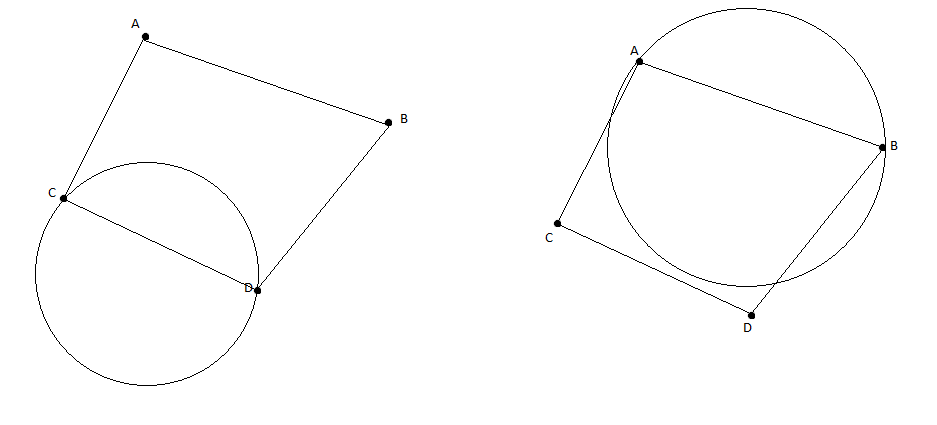
\includegraphics{Figure.png}
\caption{Figure 1: For describing 4 point problem}
\end{figure}

\begin{figure}
\centering
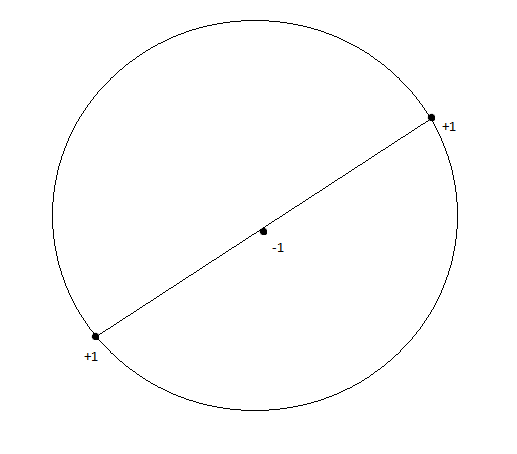
\includegraphics{Figure2.png}
\caption{Figure 2: Explaining a special case for our question.}
\end{figure}

    % Add a bibliography block to the postdoc
    
    
    
    \end{document}
